\documentclass{article}
\usepackage[utf8]{inputenc}
% -------------------- Packages --------------------
\usepackage{amsmath}
\usepackage{amssymb}
\usepackage[noend]{algpseudocode}
\usepackage{algorithm}
\usepackage{graphicx}
\usepackage{float}
\usepackage{fontawesome5}
\usepackage{listings}

\lstset{language=Python,keywordstyle={\bfseries \color{blue}}}
\NewDocumentCommand{\codeword}{v}{%
    \texttt{\textcolor[HTML]{5c5c65}{#1}}%
}


\usepackage{hyperref}
\hypersetup{
    colorlinks=true,
    linkcolor=blue,
    filecolor=magenta,      
    urlcolor=cyan,
    pdftitle={Overleaf Example},
    pdfpagemode=FullScreen,
    }

\urlstyle{same}

\usepackage{bookmark}
\hypersetup{hidelinks} %enlève les cadres rouges autour des hyperliens


% ---------- PSEUDO CODE : hack to remove indent ----------
% https://tex.stackexchange.com/questions/354564/how-to-remove-leading-indentation-from-algorithm
\usepackage{xpatch}
\makeatletter
\xpatchcmd{\algorithmic}
  {\ALG@tlm\z@}{\leftmargin\z@\ALG@tlm\z@}
  {}{}
\makeatother

\usepackage{xcolor}
\usepackage[framemethod=tikz]{mdframed}
\usepackage{tikzpagenodes}
\usetikzlibrary{calc}


% add foreach
\algnewcommand\algorithmicforeach{\textbf{for each}}
\algdef{S}[FOR]{ForEach}[1]{\algorithmicforeach\ #1\ \algorithmicdo}



% -------------------- Couleurs --------------------
\definecolor{definition}{HTML}{2f80ed}
\definecolor{definition-bg}{HTML}{e0ecfd}

\definecolor{danger-color}{HTML}{e6505f}
\definecolor{danger-bg-color}{HTML}{fce5e7}



\definecolor{gris-color}{HTML}{dadce0}
\definecolor{blanc-color}{HTML}{fcfcfc}

% -------------------- Styles --------------------



% -------------------- Macros --------------------
\mdfdefinestyle{definition-style}{%
  innertopmargin=10px,
  innerbottommargin=10px,
  linecolor=definition,
  backgroundcolor=definition-bg,
  roundcorner=4px
}
\newmdenv[style=definition-style]{definition}

\newcommand\testos[1]{clovis{\MakeUppercase #1}}

\newcommand\clovisColorfulBlock[1]{
    % #1 = danger (name)
    % #2 = danger-color (color)
    % #3 = danger-bg-color (background color)
    \mdfdefinestyle{#1-style}{%
        innertopmargin=10px,
        innerbottommargin=10px,
        linecolor=#1-color,
        backgroundcolor=#1-bg-color,
        roundcorner=4px
    }
    \newmdenv[style=#1-style]{#1}

    
    \expandafter\newcommand\csname clovis#1\endcsname[1]{
        \begin{#1}
        {\scriptsize \textcolor{#1-color}{\faIcon{exclamation-triangle} \textbf{DANGER}}}
        \vspace{3px}
        \\ ##1
        \end{#1}
    }
}

\clovisColorfulBlock{danger}

\newcommand\clovisDefinition[2]{
    \begin{definition}
    { \scriptsize \textcolor{definition}{\faIcon{graduation-cap} \textbf{DEFINITION}}}
    \vspace{3px}
    \\ \underline{\textbf{#1}}
    \vspace{2.5px}
    \\ #2
    \end{definition}
}

\newcommand\tab{\hspace*{14px}}

% -------------------- Test color box --------------------
\usepackage[most]{tcolorbox}
\tcbset{on line, 
        boxsep=3px, left=0pt,right=0pt,top=0pt,bottom=0pt,
        boxrule=0.5px,
        colframe=gris-color,colback=blanc-color,  
        highlight math style={enhanced}
        }

\newcommand\code[1]{\tcbox{{\small\tt #1}}}

% -------------------- Document --------------------
\title{Algorithmique\\De l'analyse à la conception}
\author{}
\date{Licence 3\\2021 - 2022}
\begin{document}
\normalsize
\maketitle

\renewcommand*\contentsname{Table des matières}
\tableofcontents
\newpage
\section{Niveaux de description \textit{de l'élégance du langage}}

\clovisDefinition{Type}{
    Un ensemble de valeurs.
}

\subsection{Caractéristiques d'un langage}
Un langage doit être :
\begin{itemize}
  \item \textbf{universel} \textit{(tout problème doit avoir une solution qui peut être programmé dans le langage)}
  \item le plus \textbf{naturel} possible
  \item \textbf{implémentable} sur un ordinateur
\end{itemize}

\clovisdanger{
La différence entre un langage naturel et un langage de programmation est l'\textbf{ambiguïté} : il ne doit y avoir qu'une seule interprétation possible.
}

\section{Types de données abstraits}
note : affectaton avec une flèche vers la gauche
\\attention : on indice les tableaux de 1 à n !!!

\subsection{Pile}
\code{Pile}
\\avec un tableau : \code{maPile.tab[]}
\\initialise taille = 0

%
méthodes :
\\- \code{pileVide()}
\\- \code{empiler(x)}
\\- \code{depiler()}
%
\\\\Algo \code{pileVide}
\\données : self.pile
\\résultat: booléen
\\début \texttt{
\\    retourner taille = 0
\\}fin
%
%
\\Algo \code{empiler(x)}
\\données : self.pile, x:monType
\\résultat: void
\\début \texttt{
\\Si (taille $<$ max):
\\\tab taille = taille + 1
\\\tab tab[taille] = x
\\}fin
%
\\\\Algo \code{depiler()}
\\données : self.pile
\\résultat: res:monType
\\début \texttt{
\\Si ($\tcbhighmath{taille} > 0$):
\\\tab res = tab[taille]
\\\tab\tab taille = taille - 1
\\\tab renvoyer res
\\}fin


\subsection{Tas}
\code{Tas}
\\avec un tableau : \code{monTas.tab[]}
attributs :
\\taille = 0
\\max

%
méthodes :
\\- \code{pere(i)}
\\- \code{fg(i)}
\\- \code{fd(i)}
\\- \code{insérer(x)}
\\- \code{extraire(i)}
%
\\\\Algo \code{tas.insérer(x)}
\\données : self.tas, x:monType
\\résultat: void
\\début \texttt{
\\\tab si ($taille < max$)
\\\tab\tab i = taille + 1
\\\tab\tab tantque ((i $\neq$ 1) et x $>$ tab[pere(i)])
\\\tab\tab\tab tab[i] = tab[pere(i)]
\\\tab\tab\tab i = pere(i)
\\\tab\tab tab[i] = x
\\\tab\tab taille = taille + 1
\\}fin


\subsection{Ensemble dynamique}
note : il faut garder l'ensemble dynamique \textbf{ordonné !}


\subsection{File de priorité}

\subsection{Collection (ou famille d'ensembles)}
Un ensemble de sous-ensembles de mon ensemble X
ex : une partition


%
\subsection{Définition de TDA}
\clovisDefinition{Type de données abstrait}{
    Un TDA est composé d'un ensemble d'objets similaires dans la forme et dans le comportement, et d'un ensemble d'opérations sur ces objets.
}
\section{Analyse et complexité}

\section{Algorithmes gloutons}

\section{Programmation dynamique}
\begin{figure}[H]
    \centering
    \scalebox{0.5}{
        %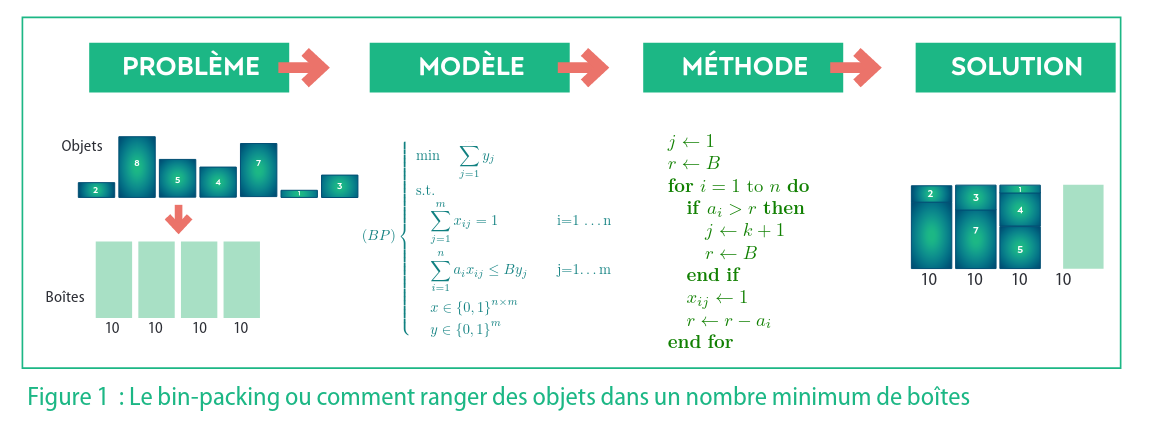
\includegraphics{img/bin-packing.png}
    }
\end{figure}

\end{document}
